\DeclareOption*{\PassOptionsToClass{\CurrentOption}{abntex2}}
\ProcessOptions

\documentclass[
	% -- opções da classe memoir --
	12pt,				% tamanho da fonte
	openright,			% capítulos começam em pág ímpar (insere página vazia caso preciso)\
	oneside,			% para impressão em verso e anverso. Oposto a oneside
	a4paper,			% tamanho do papel. 
	% -- opções da classe abntex2 --
	chapter=TITLE,		% títulos de capítulos convertidos em letras maiúsculas
	%section=TITLE,		% títulos de seções convertidos em letras maiúsculas
	%subsection=TITLE,	% títulos de subseções convertidos em letras maiúsculas
	%subsubsection=TITLE,% títulos de subsubseções convertidos em letras maiúsculas
	% -- opções do pacote babel --
	english,			% idioma adicional para hifenização
	french,				% idioma adicional para hifenização
	spanish,			% idioma adicional para hifenização
	brazil				% o último idioma é o principal do documento
	]{abntex2}

\usepackage{conf-ifsc}	

%---------------------------------------------------------------------%
%---------------------------------------------------------------------%
% Informações de dados para CAPA e FOLHA DE ROSTO
%---------------------------------------------------------------------%
%---------------------------------------------------------------------%

\titulo{Calibração de equipamento SDR}

\autor{Leonardo Santiago Benitez Pereira}

\local{Florianópolis}

\data{2022}

%\orientador[Orientador:\\]{Luis Carlos Martinhago Schlichting}
\orientador[Professor:\\]{Luis Carlos Martinhago Schlichting}

%\coorientador[Coorientador:\\]{Joabel Moia}

%\tipotrabalho{Monografia (Graduação)}

% O preambulo deve conter o tipo do trabalho, o objetivo, o nome da instituição e a área de concentração 
%\preambulo{Trabalho de conclusão de curso submetido ao Instituto Federal de Educação, Ciência e Tecnologia de Santa Catarina como parte dos requisitos para obtenção do título de engenheiro eletrônico}
\preambulo{}


%\textoaprovacao{Este Trabalho foi julgado adequado para obtenção do Título de Engenheiro Eletrônico em março de 2021 e aprovado na sua forma final pela banca examinadora do Curso de Engenharia Eletrônica do instituto Federal de Educação Ciência, e Tecnologia de Santa Catarina.}


%---------------------------------------------------------------------%
% Início do documento
%---------------------------------------------------------------------%

\begin{document}

\selectlanguage{brazil}
\frenchspacing 


% ----------------------------------------------------------
% ELEMENTOS PRÉ-TEXTUAIS
% ----------------------------------------------------------
% \pretextual

\imprimircapa
%\imprimirfolhaderosto* %(o * indica que haverá a ficha bibliográfica)

%---------------------------------------------------------------------%
% ATENÇÃO - Pergunte para a Biblioteca do IFSC
% Inserir a ficha bibliografica - 
%
% Para gerar a ficha catalográfica acesse:
% http://ficha.florianopolis.ifsc.edu.br/
% Precisa ser feito pelo navegador Mozilla Firefox
%---------------------------------------------------------------------%

%\imprimirficha{template/fichacatalografica3.pdf}
%\cleardoublepage

%---------------------------------------------------------------------%
% Inserir folha de aprovação
%---------------------------------------------------------------------%

%\imprimiraprovacao
%\cleardoublepage

%---------------------------------------------------------------------%
% Dedicatória
%---------------------------------------------------------------------%
%\imprimirdedicatoria{Este trabalho é dedicado às crianças adultas que,\\quando pequenas, sonharam em se tornar cientistas.}
% ---

%---------------------------------------------------------------------%
% Agradecimentos
%---------------------------------------------------------------------%
%\begin{agradecimentos}
%    ...
    %\marcador{add}{Tanta gente...}
%\end{agradecimentos}
% ---

%---------------------------------------------------------------------%
% Epígrafe
%---------------------------------------------------------------------%
%\begin{epigrafe}
%    \vspace*{\fill}
%	\begin{flushright}
%		\textit{``Eu não falhei, encontrei 10 mil\\
%		soluções que não davam certo.'' \\
%		(Thomas A. Edison)}
%	\end{flushright}
%\end{epigrafe}

%---------------------------------------------------------------------%
% RESUMOS
%---------------------------------------------------------------------%
% resumo em português
%\setlength{\absparsep}{18pt} % ajusta o espaçamento dos parágrafos do resumo
%\begin{resumo}
%    ...
%    \textbf{Palavras-chave}: Compatibilidade eletromagnética. Eletrônica de potência. Buck \interleaved. Conversor Buck com célula de comutação de três estados.
%\end{resumo}

% resumo em inglês
%\begin{resumo}[Abstract]
% \begin{otherlanguage*}{english}
%    ...

%   \vspace{\onelineskip}
 
%   \noindent 
%   \textbf{Keywords}: Eletromagnetic compatibility. Power eletronics. Buck Interleaved. Three-state switching cell Buck Converter.
% \end{otherlanguage*}
%\end{resumo}


%---------------------------------------------------------------------%
% inserir lista de ilustrações
%---------------------------------------------------------------------%
\pdfbookmark[0]{\listfigurename}{lof}
\listoffigures*
\cleardoublepage

%---------------------------------------------------------------------%
% inserir lista de tabelas
%---------------------------------------------------------------------%
%\pdfbookmark[0]{\listtablename}{lot}
%\listoftables*
%\cleardoublepage

%---------------------------------------------------------------------%
% inserir lista de listings
%---------------------------------------------------------------------%
%\pdfbookmark[0]{\lstlistlistingname}{lol}
%\listoflistings
%\cleardoublepage

%---------------------------------------------------------------------%
% inserir lista de abreviaturas e simbolos
%---------------------------------------------------------------------%
%\listofabrev{tex/00-Abreviaturas}
%\imprimirlistadeabreviaturas
%\imprimirlistadesimbolos
%\cleardoublepage

%---------------------------------------------------------------------%
% inserir o sumario
%---------------------------------------------------------------------%
\pdfbookmark[0]{\contentsname}{toc}
\tableofcontents*
\cleardoublepage

% ----------------------------------------------------------
% ELEMENTOS TEXTUAIS
% ----------------------------------------------------------
\textual

% ----------------------------------------------------------
% Inclusão dos capítulos que estão em outros arquivos .tex
% ----------------------------------------------------------

%%%%%%%%%%%%%%%%%%%%%%%%%%%%%%%%%%%%%%%%%%%%%%%%%%%%%%%%%%%%%%%%%%%
%%%%%%%%%%%%%%%%%%%%%%%%%%%%%%%%%%%%%%%%%%%%%%%%%%%%%%%%%%%%%%%%%%%
\chapter{Introdução}
%%%%%%%%%%%%%%%%%%%%%%%%%%%%%%%%%%%%%%%%%%%%%%%%%%%%%%%%%%%%%%%%%%%
%%%%%%%%%%%%%%%%%%%%%%%%%%%%%%%%%%%%%%%%%%%%%%%%%%%%%%%%%%%%%%%%%%%
Um dos equipamentos mais importantes para a análise de Compatibilidade Eletromagnética é o analisador de espectro, capaz de - entre outros - medir a densidade de potência espectral (\textit{power spectral density} - PSD) de um sinal \cite{aulaSpirroEMC}. Tal equipamento possui alto custo, porém pode ser substituido por rádios definidos por software (\textit{software defined radio} - SDR) \cite{tccIgor}.

Este relatório descreve o processo de calibração e ajuste dos valores de amplitude de um SDR RSP1, onde considerou-se como "valor real"\  as medições realizadas com o analisador de espectro Rohde \& Schwarz HMS-X. O trabalho foi realizado como parte da disciplina de Tópicos Avançados em Compatibilidade Eletromagnética do curso de Engenharia Eletrônica do Instituto Federal de Educação, Ciência e Tecnologia de Santa Catarina.

\chapter{Objetivos}

\textbf{Objetivos gerais}: 
\begin{itemize}
    \item Realizar a calibração e ajuste de um SDR RSP1.
\end{itemize}



\textbf{Objetivos específicos}:
\begin{itemize}
\item Realizar medições com os equipamentos SDR RSP1 e R\&S HMS-X na faixa de 10MHz a 200MHz;
\item Determinar o erro sistemático do SDR RSP1 em relação ao R\&S HMS-X para as frequências medidas;
\item Identificar se o erro é dependente da frequência;
\item Determinar o fator de ajuste necessário para corrigir o erro sistemático do SDR RSP1;
\item Determinar a incerteza das medições realizadas com o equipamento SDR RSP1.
\end{itemize}





%%%%%%%%%%%%%%%%%%%%%%%%%%%%%%%%%%%%%%%%%%%%%%%%%%%%%%%%%%%%%%%%%%%
%%%%%%%%%%%%%%%%%%%%%%%%%%%%%%%%%%%%%%%%%%%%%%%%%%%%%%%%%%%%%%%%%%%
\chapter{Desenvolvimento}

%%%%%%%%%%%%%%%%%%%%%%%%%%%%%%%%%%%
\section{Revisão de Literatura}

\subsection{Calibração}
Estabelece o erro de medição e a incerteza de medição associada de
um instrumento, ao compará-lo a um padrão \cite{slidesCalibracaoLacen}.


Segundo \citeonline{VIM}, uma calibração pode ser expressa por meio de uma declaração, uma função de calibração, um diagrama de calibração, uma curva de calibração ou uma tabela de calibração.

\citeonline{vidotto2022} aponta que o processo de calibração de SDRs pode ser feito tanto para recepção quanto emissão, sendo que ambos podem ser realizados pela comparação com um equipamento de referência.


\subsection{Ajuste}
Operação destinada a levar um instrumento de medição a um funcionamento adequado à sua utilização \cite{slidesCalibracaoPaulo}. Após o ajuste físico ou manutenção de um instrumento ou sistema de medição, tal instrumento ou sistema de medição deve ser calibrado novamente \cite{slidesCalibracaoLacen}.

Diversos tipos de ajuste de um sistema de medição incluem o ajuste de zero, o
ajuste de defasagem (às vezes chamado ajuste de "\textit{offset}") e o ajuste de amplitude (às vezes chamada ajuste de ganho) \cite{VIM}.


\citeonline{VIM} ressalta a importância de não confundir a calibração com o ajuste de um sistema de medição, frequentemente denominado de maneira imprópria de "auto-calibração": O processo de ajuste elimina, total o parcialmente, o erro, mas a medição ainda possui incerteza.


\subsection{Erro}
Estabelece o quanto o resultado da medição de um instrumento se desviou
do valor nominal \cite{slidesCalibracaoLacen}.

Segundo \citeonline{VIM}, o conceito de erro de medição pode ser utilizado quando:
\begin{enumerate}
\item existe um único valor de referência, o que ocorre se uma calibração for realizada por meio de um padrão de medição com um valor medido cuja incerteza de medição é desprezável, ou se um valor convencional for fornecido; nestes casos, o erro de medição é conhecido;
\item se suponha que um mensurando é representado por um único valor verdadeiro ou um conjunto de valores verdadeiros de amplitude desprezável; neste caso, o erro de medição é desconhecido.
\end{enumerate}

\subsection{Incerteza}
Indica a faixa em que o "valor real"\ (valor verdadeiro convencional) pode estar \cite{slidesCalibracaoLacen}. É necessariamente um valor real não-negativo, representado pelo simbolo $u$, e caracteriza a dispersão dos valores atribuídos a um
mensurando \cite{VIM}.

Há duas abordagens na estimativa da incerteza de medição $u$:
tipo A e tipo B. A incerteza do tipo A é estimada a partir da
distribuição estatística dos valores \cite{slidesCalibracaoPaulo}.

$$
u_{tipo-A} = \text{desvio padrão} / sqrt(N)
$$

$$
\text{desvio padrão} = \sqrt{\frac{\sum(x_i - \bar{x})^2}{N-1}}
$$

$$
\text{N = Número de amostras}
$$

% se eu medir 10V e u=1, eu posso escrever a medida como sendo 10+-1, o que significa que há 68% de probabilidade do valor real estar entre 9 e 11 (o 68% vêm do 1 descrio padrão)

A incerteza do tipo B não é calculada de forma estatística, mas sim em especificações de fabricantes, em informações de publicações científicas, entre outros \cite{slidesCalibracaoPaulo}. Formas usuais de quantificar as incertezas do tipo B são: metade da menor divisão de escala (para equipamentos analógicos), resolução (para equipamentos digitais), valores publicados por autoridade competente, entre outros \cite{VIM}.



Incertezas-padrão, sejam elas do tipo A ou do tipo B, podem ser combinadas através de soma quadrática \cite{slidesCalibracaoPaulo}.

$$
u_c = \sqrt{u_1^2 + u_2^2 + ...}
$$

%%%%%%%%%%%%%%%%%%%%%%%%%%%%%%%%%%%
\section{Metodologia}
Montou-se um ambiente com o gerador de funções AFG3021B da Tektronix, uma placa de circuito impresso, uma antena de campo magnético, e um analisador de espectro (hora o SDR RSP1, hora o Rohde \& Schwarz HMS-X). Para ambos os analisadores utilizou-se os mesmos cabos, porém foi necessário utilizar um adaptador miniSMA-para-SMA para o Rohde \& Schwarz).

%Lalal (Figura \ref{fig:antena}). 

\begin{figure}[H]
    \centering
    \caption{Setup para as medições com o Rohde \& Schwarz HMS-X}
    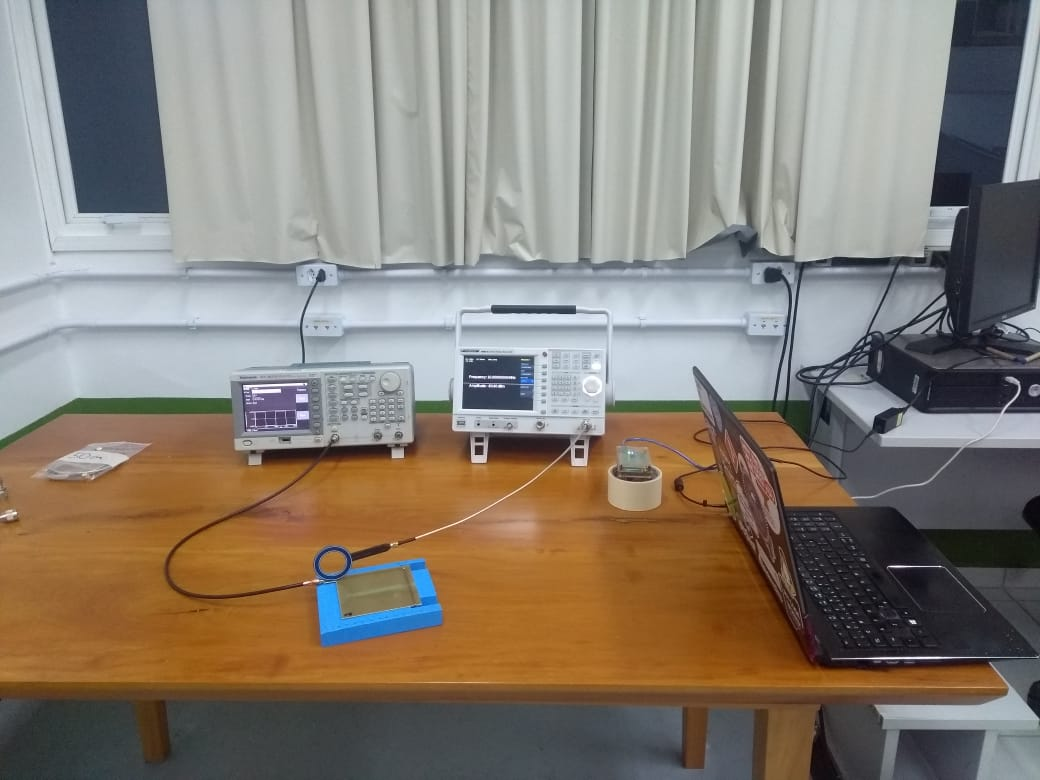
\includegraphics[width=0.4\linewidth]{Images/setup-analisador.jpeg}
    \label{fig:analisador}
\end{figure}

\begin{figure}[H]
    \centering
    \caption{Setup para as medições com o SDR RSP1}
    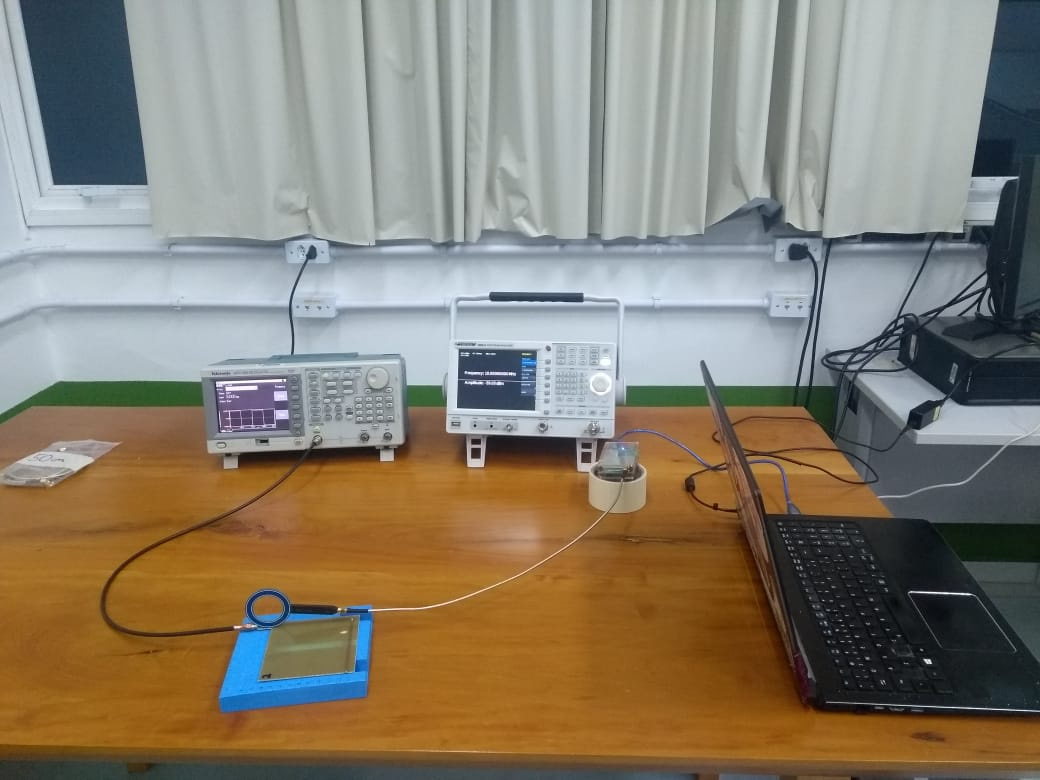
\includegraphics[width=0.4\linewidth]{Images/setup-sdr.jpeg}
    \label{fig:sdr}
\end{figure}

\begin{figure}[H]
    \centering
    \caption{Antena e posicionamento utilizados em todas as medições}
    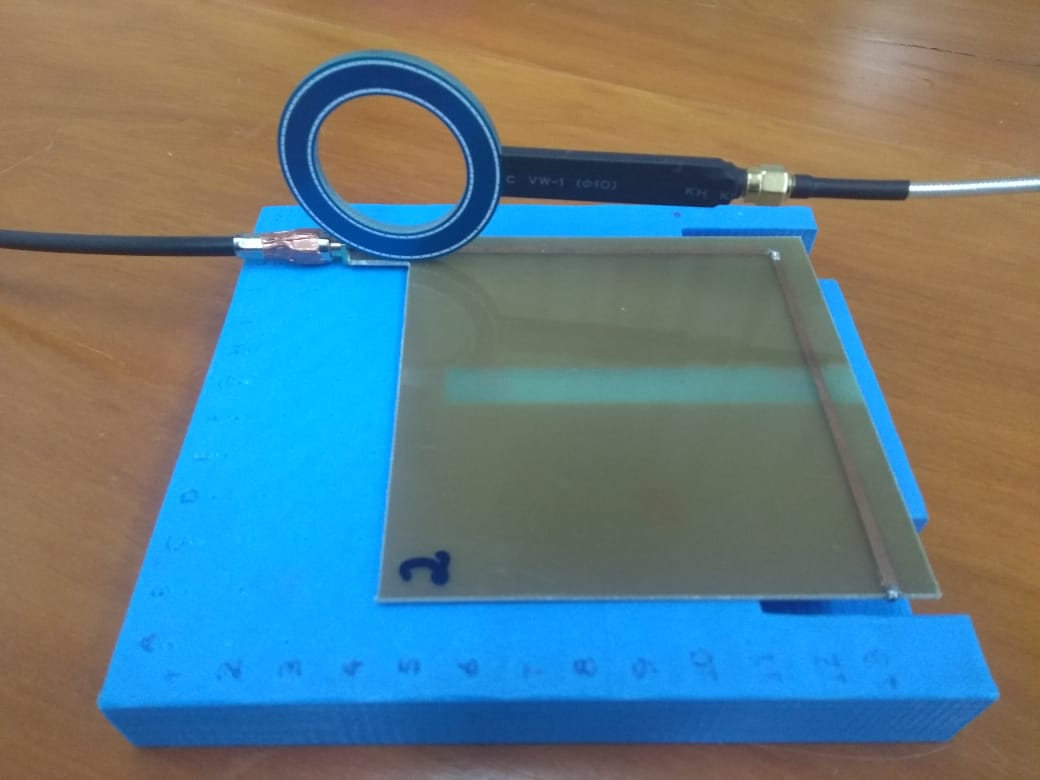
\includegraphics[width=0.4\linewidth]{Images/antena.jpeg}
    \label{fig:antena}
\end{figure}

Seguindo as instruções fornecidas em \cite{tccIgor}, o SDR RSP1 foi configurado da seguinte forma:
\begin{itemize}
    \item Ganho 1;
    \item Taxa de amostragem 1MHz;
    \item Tempo de aquisição 0,2s;
    \item Ao configurar o equipamento para medir uma determinada frequência (por exemplo, 10MHz), ajustou-se a frequência central de medição para que \textit{não} coincidisse com a frequência desejada (por exemplo, ajustando-a para 10.2MHz), eliminando assim a influência do nível DC na medição do SDR;
    \item Ao realizar a medição considerou-se apenas o valor máximo de amplitude dentro da janela de aquisição.
\end{itemize}

O analisador de espectro Rohde \& Schwarz HMS-X foi configurado da seguinte forma:

\begin{itemize}
    \item \textit{Receiver Mode} (medição de apenas uma frequência, em oposição ao \textit{Sweep Mode});
    \item Tempo de aquisição 0,2s;
    \item \textit{Peak detector};
    \item \textit{Step} de 1MHz.
\end{itemize}

Objetivando mensurar o erro e a incerteza do tipo A, realizou-se dois conjuntos de medições: 
\begin{enumerate}
    \item Medições de 10MHz a 200MHz espaçadas 10MHz entre si, para mensurar o erro;
    \item Medições de 10Mhz a 200Mhz espaçadas 50MHz entre si, repetindo cada medição 10 vezes, para mensurar a incerteza.
\end{enumerate}

Após essas medições, determinou-se um fator de ajuste, nomeado alfa, que deve ser multiplicado com a medição do SDR para obter-se o valor real da medição. Da mesma forma, obteve-se o fator $u$ que quatifica a incerteza padrão da medição.





\section{Apresentação dos Resultados}
\subsection{Conjunto de medições 1}

Gerou-se uma onda quadrada com amplitude de 8V e segui-se o procedimento apresentado na Metodologia. Como só existem as harmônicas pares, uma a cada duas medições era apenas o nível de ruído de fundo sendo medido. Calculou-se separadamente o fator de correção alfa para as amostras onde havia uma sinal presente (10Mhz, 30MHz, etc) e quando não havia um sinal presente (20MHz, 40MHz, etc).
\begin{table}[H]
    \centering
    \begin{tabular}{|l|l|l|l|l|}
    \hline
        Freq. (MHz) & Pico R\&S (dBm) & Pico SDR (dBm) & Alfa sinal & Alfa fundo \\ \hline
        10 & -34.08 & -29.93 & 1.14 & ~ \\ \hline
        20 & -71.75 & -68.89 & ~ & 1.04 \\ \hline
        30 & -42.25 & -40.55 & 1.04 & ~ \\ \hline
        40 & -69.81 & -68.70 & ~ & 1.02 \\ \hline
        50 & -45.84 & -45.74 & 1.00 & ~ \\ \hline
        60 & -69.73 & -62.71 & ~ & 1.11 \\ \hline
        70 & -56.76 & -37.63 & 1.51 & ~ \\ \hline
        80 & -71.53 & -64.51 & ~ & 1.11 \\ \hline
        90 & -68.01 & -57.81 & 1.18 & ~ \\ \hline
        100 & -71.84 & -68.83 & ~ & 1.04 \\ \hline
        110 & -71.73 & -68.65 & 1.04 & ~ \\ \hline
        120 & -72.16 & -65.54 & ~ & 1.10 \\ \hline
        130 & -71.98 & -59.61 & 1.21 & ~ \\ \hline
        140 & -72.23 & -64.09 & ~ & 1.13 \\ \hline
        150 & -72.87 & -59.57 & 1.22 & ~ \\ \hline
        160 & -73.09 & -68.63 & ~ & 1.07 \\ \hline
        170 & -72.44 & -68.93 & 1.05 & ~ \\ \hline
        180 & -71.22 & -68.69 & ~ & 1.04 \\ \hline
        190 & -70.87 & -68.98 & 1.03 & ~ \\ \hline
        200 & -71.49 & -69.13 & ~ & 1.03 \\ \hline
    \end{tabular}
\end{table}

%TODO: ver com o spirro se esse fator é aditivo ou multiplicativo

Como as harmônicas de uma onda quadrada possuem valor decrescente com a frequência, é esperado que os valores medidos para as frequências com harmônica não-nula sejam decrescentes. Observa-se também que as medições dos equipamentos se torna mais próxima com o aumento da frequência, convergindo para um valor de aproximadamente -70dB de ruído de fundo.

\subsection{Conjunto de medições 2}
Gerou-se uma onda quadrada com amplitude de 10V e segui-se o procedimento apresentado na Metodologia.

\begin{table}[H]
    \centering
    \begin{tabular}{|l|l|l|l|}
    \hline
        Freq (MHz) & u-tipo-A SDR & u-tipo-A R\&S & Fator de correção sinal médio \\ \hline
        10 & 0.02 & 0.005 & 1.14 \\ \hline
        50 & 0.04 & 0.02 & 1.01 \\ \hline
        100 & 0.08 & 0.2 & 1.04 \\ \hline
        150 & 0.04 & 0.2 & 1.21 \\ \hline
        200 & 0.08 & 0.2 & 1.04 \\ \hline
    \end{tabular}
\end{table}

Pode-se observar que ambos os equipamentos apresentam a incerteza positivamente correlacionada com a frequência de amostragem. 

Para as medições acima de 100 MHz o equipamento R\&S apresentou uma incerteza maior. É possível que tal se deva pela forma como as medições foram realizadas: enquanto as medições com o SDR foram realizadas com menos de um segundo de intervalo de tempo entre medições subsequêntes (devido ao procedimento de medição haver sido implementado em software), as medições com o R\&S foram realizadas manualmente e, portanto, houve um intervalo de alguns segundos entre uma medição e outra.
\chapter{Conclusões}

Neste trabalho comparou-se as medidas obtidas com os equipamentos R\&S HMS-X e SDR RSP1, para a faixa de frequência de 10MHz à 200MHz.
Obteve-se o erro sistemático do SDR RSP1 em relação ao R\&S HMS-X, do qual determinou-se o o fator de ajuste necessário para corrigir o erro. Obteve-se também a incertezado tipo A do equipamento. 


Como ambos - ajuste e incerteza - são dependentes da frequência, implementou-se um código na linguagem Python que, dado uma medição, realiza o ajuste e indica a incerteza (disponível no Apêndice A). Para tanto, o código utiliza a interpolação linear dos valores obtidos para o alpha e $u$. 



% ----------------------------------------------------------
% Referências bibliográficas
% ----------------------------------------------------------
\bibliography{Bibliography/bib_electronics.bib}

% ----------------------------------------------------------
% Apêndices
% ----------------------------------------------------------
\begin{apendicesenv}
    \partapendices
    \chapter{Código de ajuste}

\begin{lstlisting}[language=Python]
import numpy as np
from typing import Tuple

adjust_table = [
  {
    'freq': 10,
    'alpha': 1.14,
    'u': 0.02,
  },
  {
    'freq': 30,
    'alpha': 1.04,
  },
  {
    'freq': 50,
    'alpha': 1.0,
    'u': 0.04,
  },
  {
    'freq': 70,
    'alpha': 1.51,
  },
  {
    'freq': 90,
    'alpha': 1.18,
  },
  {
    'freq': 100,
    'u': 0.08,
  },
  {
    'freq': 110,
    'alpha': 1.04,
  },
  {
    'freq': 130,
    'alpha': 1.21,
  },
  {
    'freq': 150,
    'alpha': 1.22,
    'u': 0.04,
  },
  {
    'freq': 170,
    'alpha': 1.05,
  },
  {
    'freq': 190,
    'alpha': 1.03,
  },
  {
    'freq': 200,
    'u': 0.08,
  },
]



def apply_adjust(frequency: float, measurement: float, adjust_table: list) -> Tuple[float, float]:
  '''
  The adjust_table is expected to be monotonically increasing in frequency
  Return the tuple (alpha, uncertainty)
  '''
  assert frequency >= adjust_table[0]['freq'], 'The device was not calibrated for this frequency range'
  assert frequency <= adjust_table[-1]['freq'], 'The device was not calibrated for this frequency range'
  alpha = np.interp(
      frequency, 
      [a['freq'] for a in adjust_table if 'alpha' in a],
      [a['alpha'] for a in adjust_table if 'alpha' in a],
  )
  uncertainty = np.interp(
      frequency, 
      [a['freq'] for a in adjust_table if 'u' in a], 
      [a['u'] for a in adjust_table if 'u' in a],
  )
  return (alpha, uncertainty)


frequency = 25
measurement = -70
alpha, uncertainty = apply_adjust(frequency, measurement, adjust_table)
print(f"At {frequency} MHz, we measured {measurement} V, which is adjusted to {measurement*alpha}+-{uncertainty} V\t\t(alpha={alpha})")
\end{lstlisting}
\end{apendicesenv}

% ----------------------------------------------------------
% Anexos
% ----------------------------------------------------------
%\begin{anexosenv}
%    \partanexos
%    \include{tex/40-Anexos}
%\end{anexosenv}

%---------------------------------------------------------------------
% INDICE REMISSIVO
%---------------------------------------------------------------------
%\phantompart
%\printindex
%---------------------------------------------------------------------

\end{document}
